\chapter{Hardware and Data Preprocessing}
\label{ch:Hardware}

As aforementioned, we used a MIMU (GaitWatch) and a force plate (Zebris FDM-S) to gather the raw gait data. In this chapter we will describe the employed hardware in detail. Subsequently, we will elaborate on the necessary synchronisation of both systems.

\section{GaitWatch}

The GaitWatch device \cite{olivares_vicente_gaitwatch_2013} is designed to monitor the motion of patients by means of inertial sensors while attached to the body. It was developed at the Department of Neurology of the Ludwig-Maximilians University in Munich in conjunction with the Department of Signal Theory, Telematics and Communications of the University of Granada. The system is composed of a set of embedded magnetic and inertial sensors wired to a box containing a microcontroller. This microcontroller is in charge of collecting data from the embedded box sensors, as well as from the external measurement units, and storing them on a memory card. The various units are placed at the patient's thighs, shanks, arms and trunk as shown in Figure \ref{fig:GaitWatch_placement}. The components of the three different kinds of subunits are described below:

\begin{figure}
	\centering
	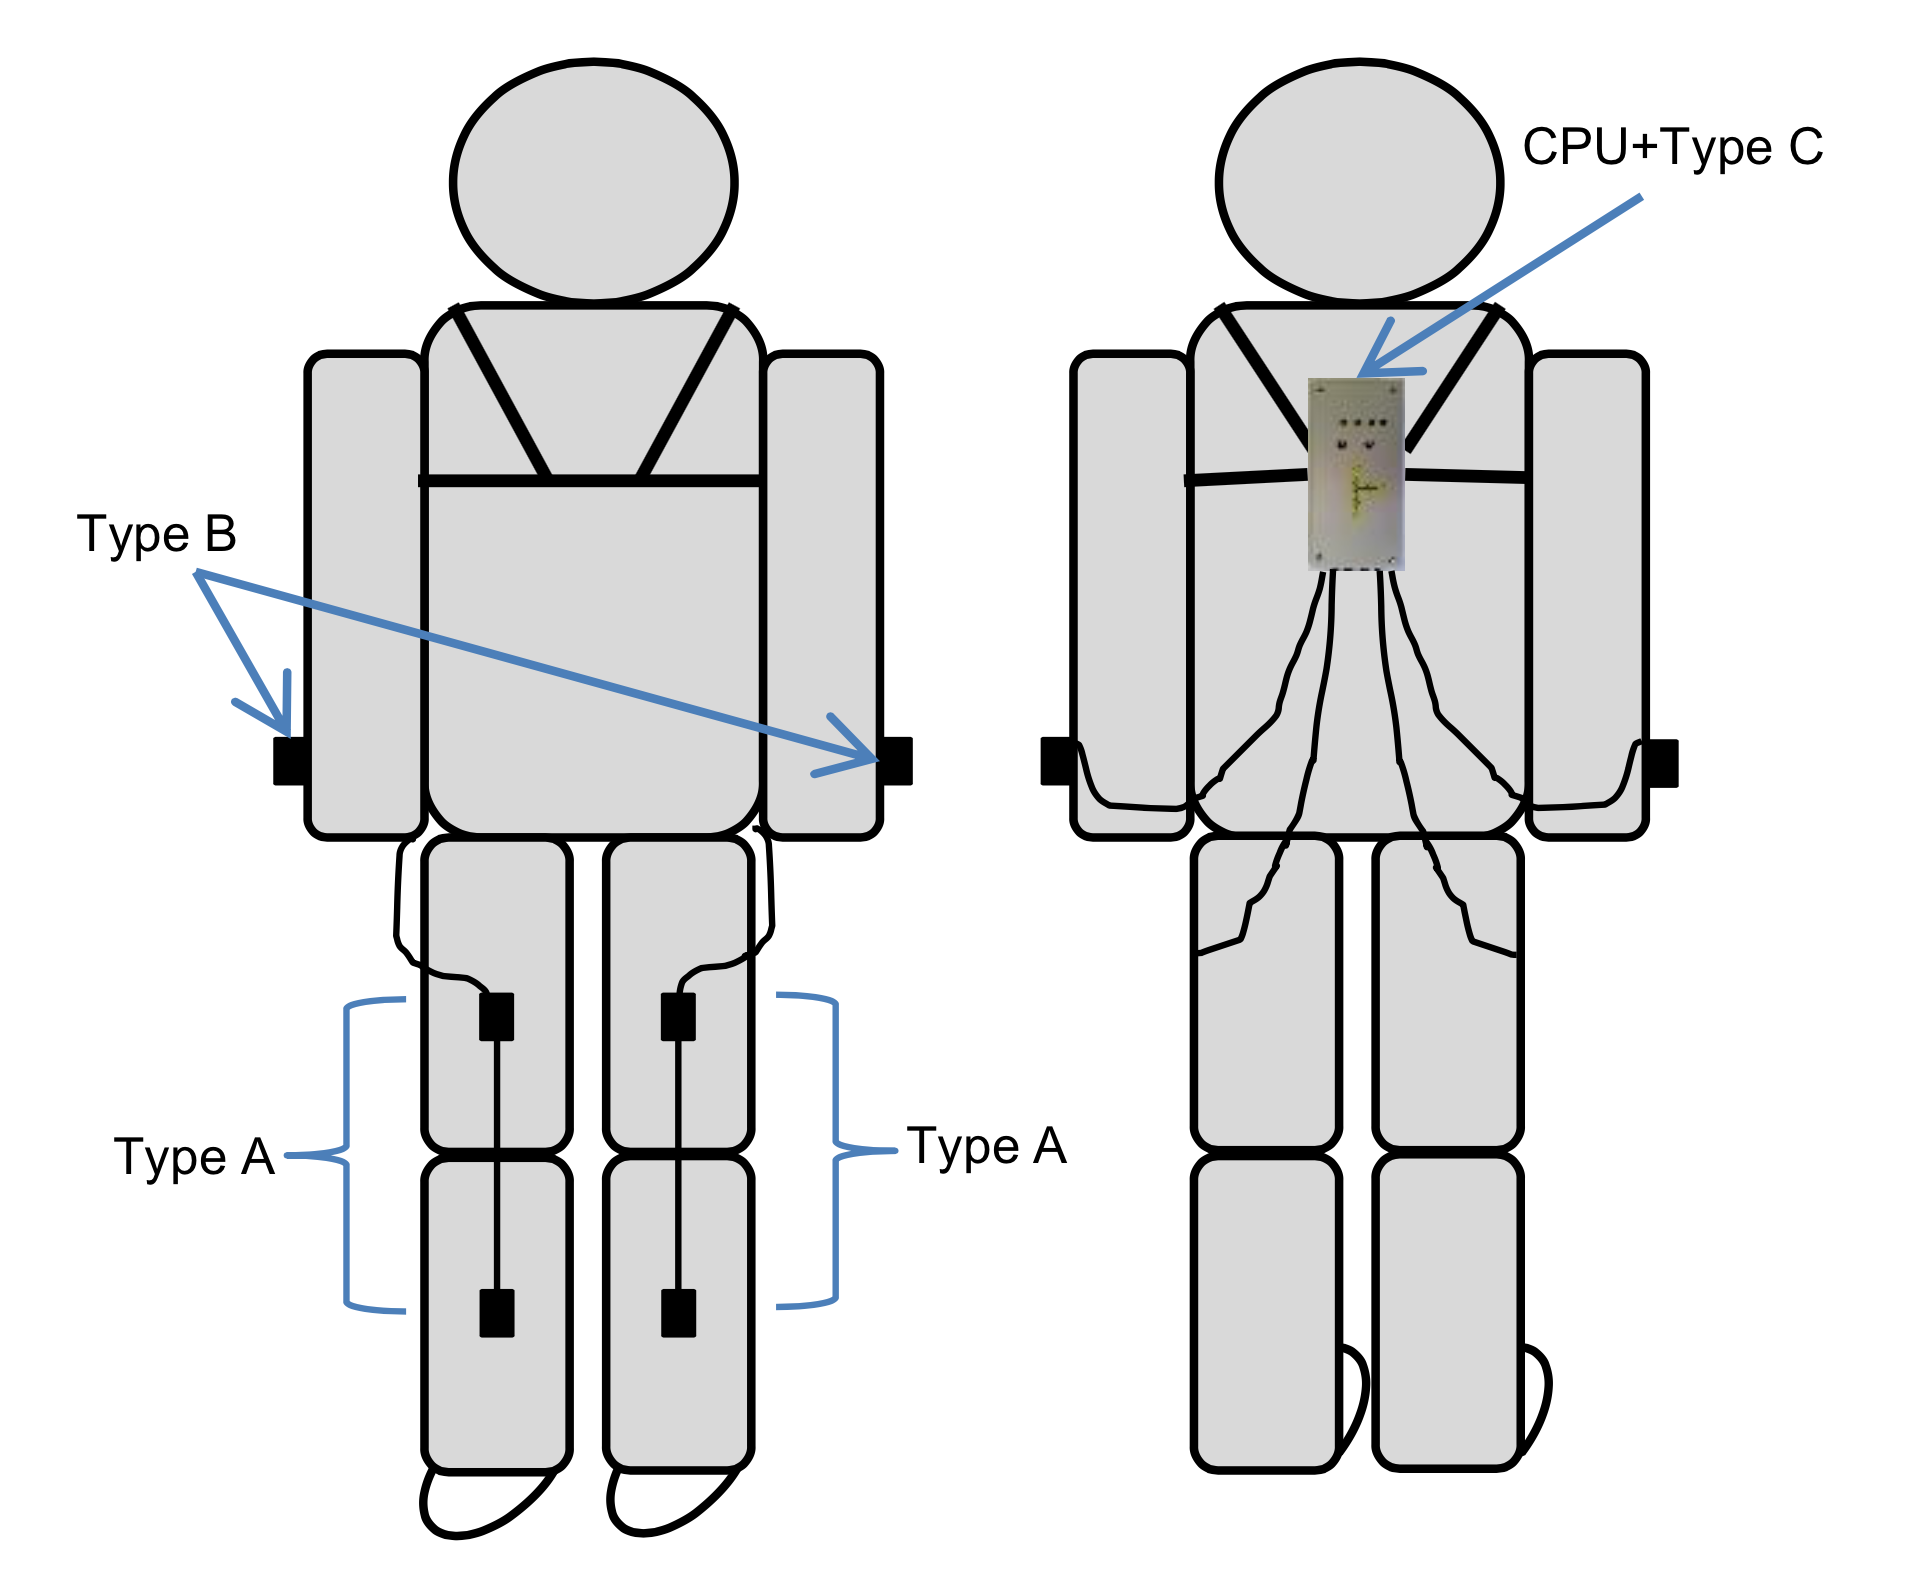
\epsfig{file=images/GaitWatch_placement, width=9cm}
	\caption{Placement of GaitWatch components at the body \cite{olivares_vicente_gaitwatch_2013}.}
	\label{fig:GaitWatch_placement}
\end{figure}

\begin{itemize}

\item \textsc{Type A} (thighs and shanks): 

IMU Analog Combo Board with 5 Degrees of Freedom from \Citeauthor{IMU5} \cite{IMU5} containing an IDG500 biaxial gyroscope (from which only Y axis is actually used) with a measurement range of ±500\,°/s \cite{IDG500} and a ±3\,g triaxial accelerometer, ADXL335 from \Citeauthor{ADXL335} \cite{ADXL335}.

\item \textsc{Type B} (arms):

IDG500 biaxial gyroscope with a measurement range of ±500\,°/s from \Citeauthor{IDG500} \cite{IDG500}.

\item \textsc{Type C} (trunk):

ADXL345 triaxial accelerometer with programmable range of ±2\,g/±4\,g/±8\,g/±16\,g from \Citeauthor{ADXL345} \cite{ADXL345},
IMU3000 triaxial gyroscope with programmable range of ±250/±500/±1000/±3000\,°/s from \Citeauthor{IMU3000} \cite{IMU3000}, 
Micromag3 triaxial magnetometer with a measurement range of ±11\,Gauss from \Citeauthor{MicroMag3} \cite{MicroMag3}, AL-XAVRB board containing an AVR ATxmega processor from \Citeauthor{AVRATxmega} \cite{AVRATxmega}.

\end{itemize}


\section{Zebris FDM-S}

The Zebris FDM-S \cite{zebris_force_plate_2013} is a force measuring plate for stance and gait analysis with a sensor area of 540 x 330 mm accommodating 40 x 64 force sensors, which results in 1.4 sensors per square centimetre and 2560 sensors in total. The data was sampled at a frequency of 120\,Hz.

\section{Synchronisation}

According to the data gathering protocol in \ref{data_gathering_protocol} the raw data that was collected with the MIMU and the force plate had distinct time axes, which is why a synchronisation of both systems was necessary. In order to achieve this we created a MATLAB$\textsuperscript{\textregistered}$ routine that read both the raw force plate and GaitWatch data, calibrated the GaitWatch signals and carried out the synchronisation for all patients in a data set.

The single data sets of each patient that we received from the clinic in Munich consisted of one .mat-file containing the GaitWatch signals and ten text files with the force plate signals of one cycle, respectively. An Excel-file for all patients of one complete data set stated the order of the separate text files, the corresponding GaitWatch .mat-file, their file names as well as additional hints and characteristics in respect of the patient, e.g. `patient with freezing' or `deep brain stimulation'. To read the force plate data in the right order and to associate the correct GaitWatch file we evaluated this Excel-file, so that the rest of the synchronisation could be automatised.

We used the z-axis of the acceleration signals of both shanks for synchronisation, since those had a large peak at the point in time when the patient touched the force plate. That was also the time when the force plate signals attained nonzero values.  First we detected the second peak pointing upwards of each separate gait cycle in the aforementioned signals. We detected the second one since when the patient initiated the step onto the force plate there was a peak pointing upwards while accelerating his leg upwards, then one pointing downwards at the point in time when the motion changes its direction and the patient lowers his leg. Finally, there was a second peak pointing upwards when the foot touches the force plate and thus the shank decelerates strongly. Patients could step with an arbitrary limb onto the force plate, in order to keep the procedure as natural as possible. As seen in the upper two graphs in Figure \ref{fig:left_right_detect} we distinguished between stepping with the left foot first and stepping with the right foot first and used the sooner peak as synchronisation line. 

\begin{figure}
	\centering
	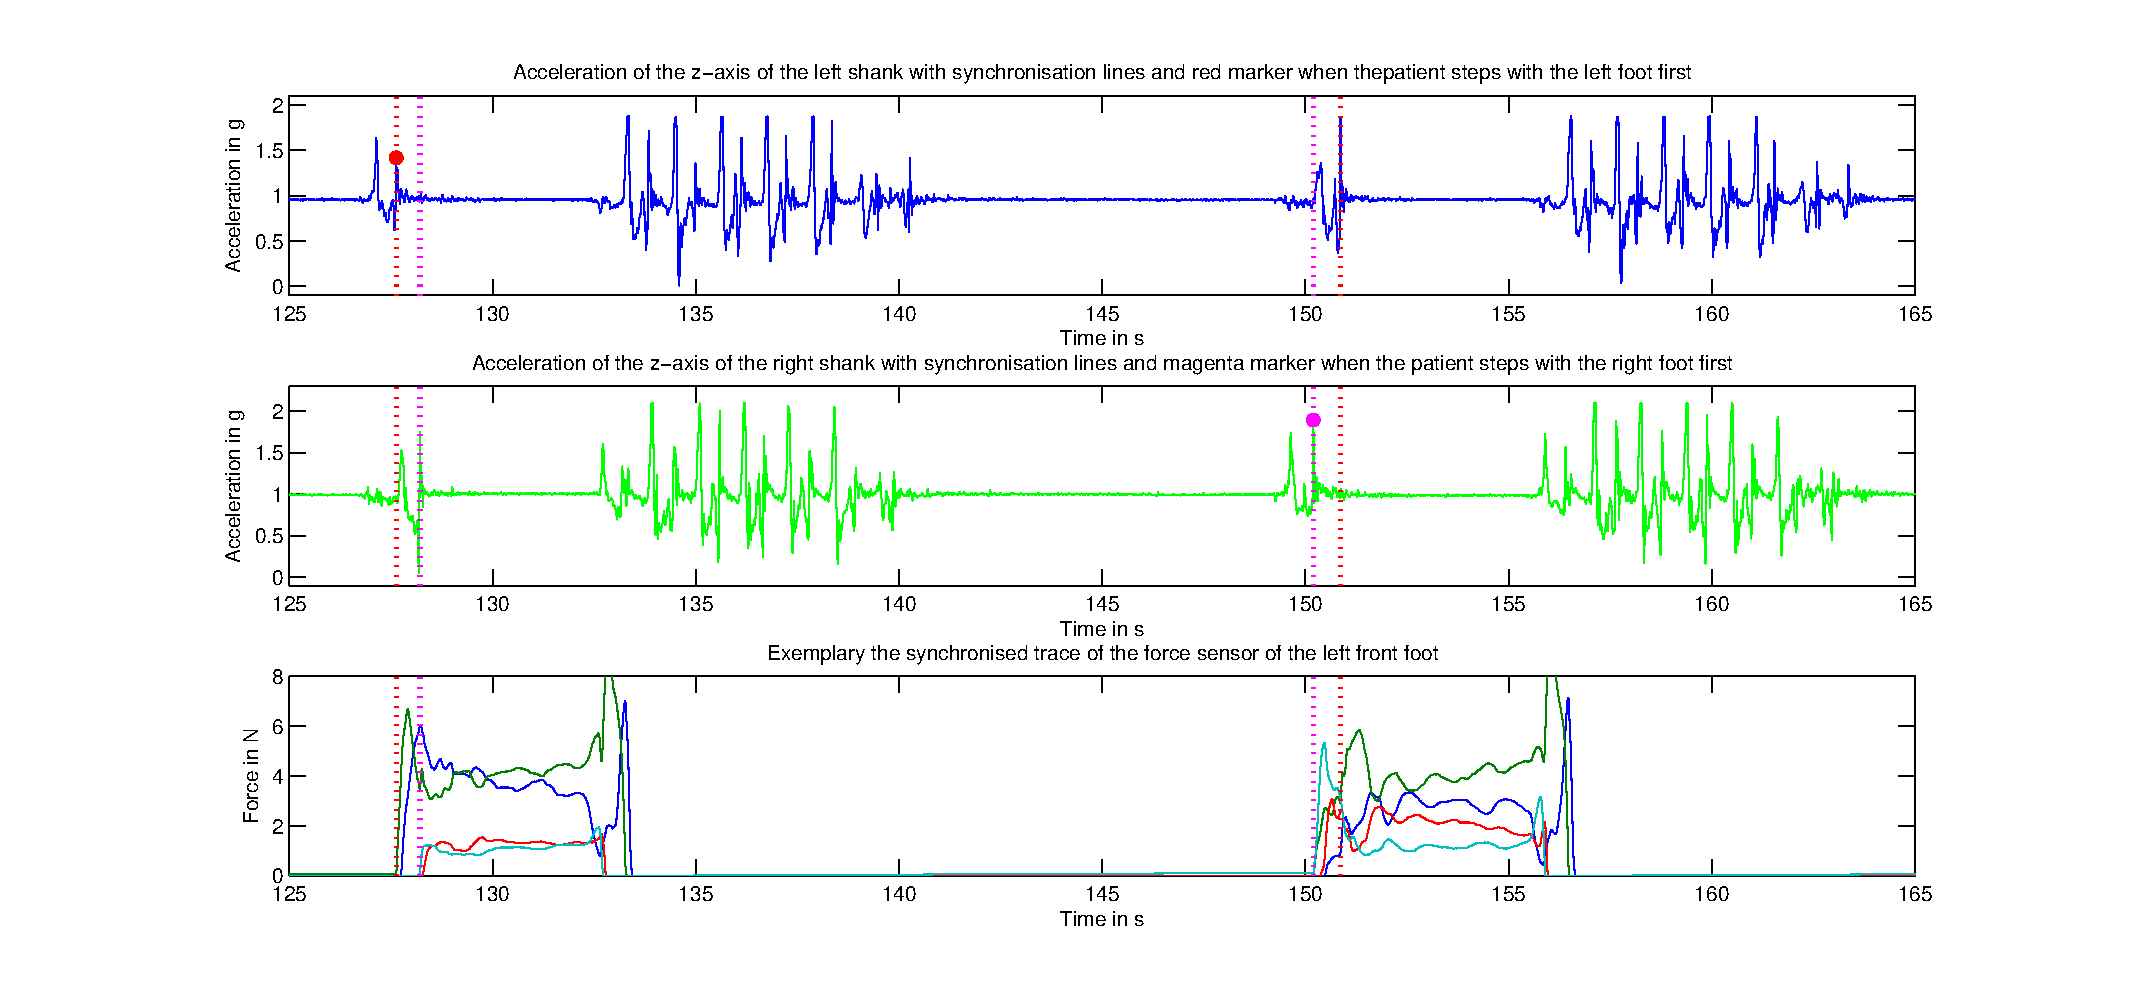
\epsfig{file=images/left_right_detect, width=16cm}
	\caption{Left-right detection of stepping limb and synchronised signals of the four force sensors.}
	\label{fig:left_right_detect}
\end{figure}

  Next, we computed the differences between the time vectors of the force plate signals and the GaitWatch signals and corrected the force plate time vector, accordingly. Then the force plate signals were resampled at the GaitWatch sampling frequency of \mbox{200 Hz}. Eventually the signals were grouped in time series objects, separated in chunks of one cycle and stored in cell arrays, in which one cell contained one cycle, as a .mat-file. The lower graph in Figure \ref{fig:left_right_detect} shows exemplary the synchronised signals of the four force sensors. 

